\chapter{Sistemas Vestíveis} 
\label{cap:wearablw_systems}

Sistemas Vestíveis podem ser definidos como dispositivos eletrônicos móveis que podem ser discretamente embutidos nos trajes do usuário, como parte da roupa ou um acessório. Diferente dos sistemas móveis convencionais, eles podem funcionar sem ou com muito pouca interferência nas atividades do usuário \citep{lukowicz2004wearable}. 

Hoje, muitos destes dispositivos vestíveis vem com uma gama de sensores embutidos que são utilizados na detecção de quedas. O tipo de sensor mais comum utilizado em \ac{FDS} é o acelerômetro, com alguns desses sistemas também utilizando o giroscópio como um sensor auxiliar. De acordo com a revisão sistemática feito por \cite{igual2013challenges}, 186 dos 197 sistemas analisados utilizam o acelerômetro como sensor principal na detecção de quedas. A utilização desde sensores em \ac{FDS} se deve muito pela popularização e o barateamento dos mesmos, além da utilização desses sensores embarcados em smartphones e smartwatches.


As seções desse capítulo são organizadas da seguinte maneira: A seção \ref{sec:sensors} descreve os principais tipos de sensores utilizados em \ac{FDS}; A \ref{sec:sensor_position} fala sobre o posicionamento de sensores, fazendo uma correlação entre o posiciomanento dos sensores e a accurâcia dos sistemas estudados; A seção \ref{sec: FDS_algorithm} fala sobre os diferentes tipos de algoritmos de detecção de quedas mostrando suas vantagens e desvantagens; Por fim, a seção \ref{sec:FDS_examples} irá mostrar exemplos de aplicações que realizam a detecção de quedas atravês de tecnologias vestíveis. 



\section{Sensores}
\label{sec:sensors}
A escolha e o bom funcionamento de sensores são uma parte essencial no bom funcionamento de sistemas de detecção de quedas. De forma geral, sensores são dispositivos que convertem fenômenos físicos em sinais elétricos. Sendo assim , eles representam a camada de comunicação entre o mundo físico e o mundo digital. 

Os dois tipo principais de sensores utilizados em sistemas de detecção de queda são o acelerômetro e o giroscópio. Eles fazem parte de um grupo chamado de \ac{MEMS}. Estes sensores são geralmente feitos de chips de silício utilizando as mesmas técnicas usadas na confecção de chips de computadores pessoais. Para que um sensor possa ser classificado como \ac{MEMS} alguma parte do seu design precisa vibrar ou se mover de alguma forma \citep{milette2012professional}. 

De forma geral tanto o acelerômetro quanto o giróscopio utilizam 3 eixos para expressar seus valores. O sistema de coordenadas utilizado é relativo a cada dispositivo. Na figura \ref{fig:axis_device} temos  exemplo do sistemas de coordenadas utilizado pelo sistema operacional Android\footnote{https://www.android.com/}. Neste sistema o ponto de origem é o centro da tela do dispositivo, quando segurado na posição vertical \citep{sensorAndroidDocs}. 

\begin{figure}[ht]
	\centering
	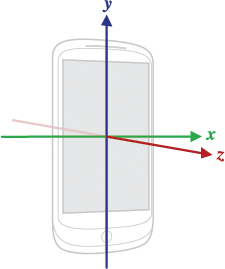
\includegraphics[scale=0.6]{imagens/axis_device.png}
	\caption{Sistema de coordenadas utilizado pelo sistema operacional Android \citep{sensorAndroidDocs}.}
	\label{fig:axis_device}
\end{figure} 

\subsection{Acelerômetro}
\label{subsec:accelerometer}
Fisicamente, o acelerômetro é um dispositivo composto de uma pequena massa  anexado a pequenas molas que são utilizadas para medir a aceleração aplicada sobre um dispositivo, incluindo a força da gravidade. A aceleração é medida analisando o quanto a massa se distancia do seu ponto de equilíbrio. 

\begin{figure}[ht]
	\centering
	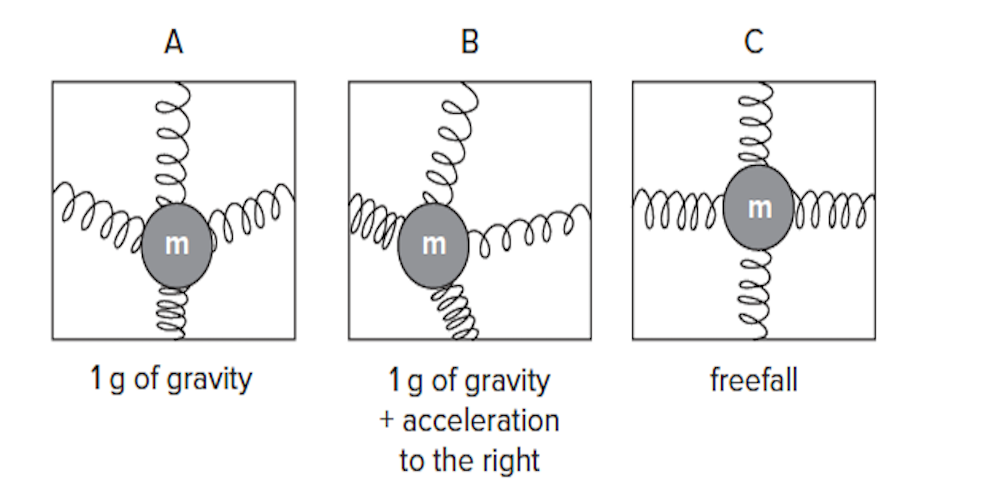
\includegraphics[scale=0.6]{imagens/MEMS_device.jpg}
	\caption{Força sendo aplicando sobre uma massa presa a molas \citep{milette2012professional}.}
	\label{fig:acelerometro}
\end{figure} 

	
Na figura \ref{fig:acelerometro} em A é possível ver um aparelho parado em uma mesa, sobre ele só irá agir a força de gravidade 1G de aproximadamente $9.8 m/s^{2}$. Em  B, o aparelho foi jogado para a direita, então irá agir sobre ele, além da força da gravidade, uma aceleração no sentido para onde o aparelho se movimentou. Já em C, vemos um aparelho em queda livre com aceleração no sentido oposto a força da gravidade, o que faz com a massa fique localizada em seu ponto de equilibrio, e a força resultante  seja de $0G$ \citep{milette2012professional}.


\subsection{Giroscópio}
	
	O giroscópio, similarmente aos acelerômetros, são pequenas massas em pequenas molas, só que em vez de medir a aceleração, são utilizados para medir um tipo de força chamada de Força de Coriolis. A Força de Coriolis é a tendência que um objeto livre possui de sair do curso quando visto de um ponto de referência em rotação \citep{milette2012professional}. Por exemplo, se sentarmos em um carrosel e rolarmos a bola pra longe, a bola irá parece desviar em uma linha reta, como se existisse uma força agindo sobre ela. Esta força é chamada de Força de Coriolis.
	
	Apesar de possuir uma estrutura física semelhante, o aceletrometro e o giroscópio se diferem em seu funcionamento. Em vez de esperar a força da gravidade agir sobre a massa, o giroscópio funciona vibrando está massa sobre o eixo definido. Quando o giroscópio é rotacionado, a Força de Coriolis faz com que a massa comece a ser mover em um eixo dirente no qual ele estava vibrando anteriomente.  \cite{milette2012professional}.
	
	Como a força de Coriolis age somente quando o dispositivo está em rotação, o giroscópio só é capaz de calcular a velocidade angular, ou seja, a velocidade com que o aparelho está sendo rotacionado. 
	
	A orientação da dispositivo irá definir quando o valor da rotação será positivo ou negativo. Nos dispositivos Android, a velocidade Angular é medida em radianos por segundo ($rad/s$) e é positiva em rotações no sentido anti-horário \citep{GyroscopeAndroidDocs}. 
	
\section{Posicionamento de Sensores}
\label{sec:sensor_position}

O posicionamento dos sensores afeta diretamente a performance dos \ac{FDS}, dependendo da posição onde colocamos os sensores, o sistema pode indicar uma maior ou menor quantidade de falhas. 

Não existe um consenso sobre a posição otimizada dos sensores para que se possa realizar a detecção de quedas. De acordo com \cite{abbate2011recognition}, a cintura seria o local ideal para o posicionamento, já que estaria mais perto do centro de gravidade do corpo humano. Entretanto em \cite{kangas2007determination}, já foi sugerido que a cabeça seria o melhor lugar para posicionar os sensores. Outras soluções, como em \cite{gjoreski2011accelerometer}, já propõem o uso de mais de um sensor, colocando-os em diferentes partes do corpo com o objetivo de aumentar ainda mais a precisão dos \ac{FDS}.


De acordo com X, o pulso não é o local recomendado para o posicionamento de sensores em sistemas de detecção de quedas. Isso se deve  a constante movimentação dos braços, que podem gerar um número grande de falso-positivos. Entretanto, alguns sistemas tem conseguido resultados satisfatórios com \ac{FDS} localizados no pulso. O sistema proposto por \cite{hsieh2014wrist}, foi capaz detectar quedas em 151 das 160 quedas simuladas e obteve uma especificidade (capacidade de não reconhecer eventos de quedas, como tal) de 95\%.

Além da acurrácia do sistema, outras questões precisam ser levadas em consideração quando pensamos no posicionamento dos sensores. Uma delas é a danificação dos sensores na occorrência de uma queda. Caso o sistema pare de funcionar, um possível alerta de emergência poderá não ser enviado e o idoso poderá está correndo grande perigo. 

Outra questão é a usabilidade, o uso de muitos sensores, apesar de poder elevar a precisão do sistema, poderá levar a um disconforto do usuário, que pode fazer até com que o mesmo desista de usá-lo. 


\section{Algoritmos de Detecção de Queda}
\label{sec: FDS_algorithm}
Os algoritmos de detecção de quedas recebem como entrada os dados obtidos através dos sensores e são capazes de determinar se o que ocorreu foi um evento de queda ou somente uma \ac{ADL}. De acordo com \cite{casilari2015analysis}, é possível separar os algoritmos de detecção em dois grandes grupos: Algoritmos de detecção através de métodos de reconhecimento de padrões, algoritmos baseados em limiares. 




\subsection{Reconhecimento de Padrões}
O reconhecimento de padrões é uma área do aprendizado de máquina que foca no reconhecimento de padrões e regularidades de dados \citep{anzai2012pattern}. Diversas técnicas de aprendizado de máquina tem sido empregadas na detecção de quedas, de acordo com a revisão sistemática feita por \cite{casilari2015analysis}, algoritmos como o de \textit{Naïve Bayes}, \textit{Redes Neurais}, e \textit{Árvores de Decisão} tem sido utilizados.


Um exemplo de sistema que utiliza a técnica de reconhecimento de padrões foi proposto por \cite{zhao2012fallalarm}. O seu algoritmo de detecção de quedas analisa dados do acelerômetro através de uma árvore de decisão, assim identificando um evento de queda. 

Este algoritmo é composto de 2 fases, a primeira é o que chamamos em aprendizado de máquina de fase de treinamento. Será realizado a coleta de dado e a  extração das características que são pertinentes, além do treinamento de um modelo de árvore de decisão. Na figura \ref{fig:decision_tree} podemos ver o modelo de árvore de decisão gerado.  Este modelo de árvore de decisão é capaz de reconhecer atividades como andar, correr, estado estático ou um evento de queda através das variáveis \textit{Std\_x}, \textit{Mean\_y} e \textit{Slope} que representam caracteristicas do sistema. 


\begin{figure}[ht]
	\centering
	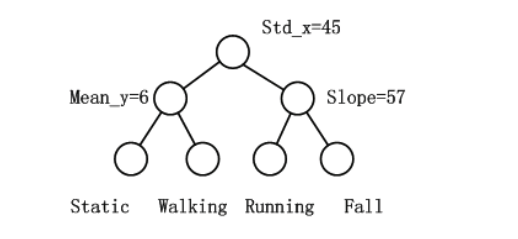
\includegraphics[scale=0.6]{imagens/decision_tree.png}
	\caption{ Modelo de árvore de decisão construida em \cite{zhao2012fallalarm}.}
	\label{fig:decision_tree}
\end{figure} 


Na segunda fase, chamada de fase de testes, o modelo de árvore de decisão é utilizado em uma aplicação no smartphone que será responsável pelo reconhecimento de atividades. Os dados dos sensores são catalogados e transformados nas caracteristicas do sistema, que serviram como dados de entrada da árvore de decisão, que terá como saída o tipo de atividade que foi desempenhada.

Sistemas que utilizam reconhecimento de padrões, normalmente está suscetível a altos custos computacionais, análise massiva de dados, e acesso a grandes bancos de dados ou longos periodos de treinamentos onde o algoritmo de classificação precisa ser parametrizado e adaptado a diferentes grupos de usuários \citep{casilari2015analysis}. Em constraste, existem os algoritmos baseados em limiares que tendem a ser mais simples e similarmente eficientes, desde que encontremos limiares adequados. 

\subsection{Baseado em Limiares}
Algoritmos baseados em limiares utilizados na detecção de quedas comparam os dados dos sensores com um ou mais valores pré-definidos, chamados de limiares. Estes valores podem ser fixos ou adaptados. Quando estes valores são adaptados, eles não mudam dinamicamente enquanto os usuários estão utilizando o sistema. Em vez disso, o usuário irá introduzir dadados sobre o seu perfil fisiológico e o sistema irá informar os limiares adequados \citep{habib2014smartphone}. Um exemplo deste tipo de sistema pode ser visto em \cite{sposaro2009ifall}, o valor limiar mudar de acordo com os parametros providos pelo usuário como altura, peso e nível de atividade. 

De acordo com a revisão sistemática feito por \cite{casilari2015analysis}, muitos sistemas de detecção de queda utilizam o valor de \ac{SMV} do vetor de aceleração como  valor limiar principal em seus algoritmos de detecção. O valor de \ac{SMV} é definido através da equação em \ref{eq:SMV}, onde $X_i$, $Y_i$, $Z_i$, representam, respectivamente, os valores de aceleração dos eixos x, y, z obtidos através do acelerômetro descrito em  \ref{subsec:accelerometer}.

\begin{equation}
SMV = \sqrt{X_i^2 + Y_i^2 + Zi_i^2} 
\label{eq:SMV}
\end{equation}

A escolha dos limiares é um fato determinante para o sucesso deste tipo de algoritmo de detecção de quedas. A escolha dos limiares pode ser feita atravês de experimentos preliminares como em \cite{zhang2013honey}. Em seu trabalho, um grupo de voluntários foi escolhido para realizar diversas \ac{ADL}, como andar, correr subir e descer escadas e também realizar a simulação de quedas. Através dos dados obtidos foi possível descobrir os limiares de \ac{SMV} para um evento de queda.  

De acordo com \cite{cao2012falld}, a performance dos algoritmos aumenta significadamente quando utilizamos valores de limiar dinâmicos. De acordo com sua pesquisa, o número de eventos de queda que não foram caracterizadas como tal, cairam de 53 para 29 quando o peso, sexo idade foram levados em consideração no momento da definição dos limiares.

Outra questão importante quando utilizado este tipo de algoritmo é o número de limiares utilizados. De acordo com \cite{casilari2015analysis}, o uso de um único limiar faz com que o algoritmo emita um número grande de alerta falsos, categorizando \ac{ADL} como eventos de queda, fazendo com que o uso de somente um limiar não seja adequado no desenvolvimento de \ac{FDS}.


\section{Trabalhos Relacionados}
\label{sec:FDS_examples}
Como vimos no decorrer desse trabalho, não existe na literatura um algoritmo ou dispositivo padrão para o desenvolvimento de \ac{FDS}. A plataforma vestível é bastante promissora por estar naturalmente aclopada a alguma parte do corpo do usuário, sendo possivel criar um algoritmo de detecção mais confiáveis, já que, como visto em \cite{casilari2015analysis}, grande parte dos algoritmos de detecção de quedas tem como pré-condição para o seu bom funcionamento, que o dispositivo esteja localizado em uma posição fixa do corpo, como cintura, pulso ou cabeça. Sendo assim, falaremos sobre três sistemas de detecção de quedas que embarcaram os seus sistemas de detecção de quedas em plataformas vestíveis. 

\subsection{SPEEDY - Detector de Quedas em um Relógio de Pulso}
SPEEDY foi o primeiro protótipo de um relógio detector de quedas construido em um smartwatch \citep{degen2003speedy}. Em seu trabalho, ele só utilizou um 2 sensores que são capazes de medir a aceleração através de 3 eixos \textit{x, y, z}. Na figura \ref{fig:speedy} é possível ver o protótipo do sistema desenvolvido e os 3 eixos utilizados para calcular o valor da aceleração. 

\begin{figure}[ht]
	\centering
	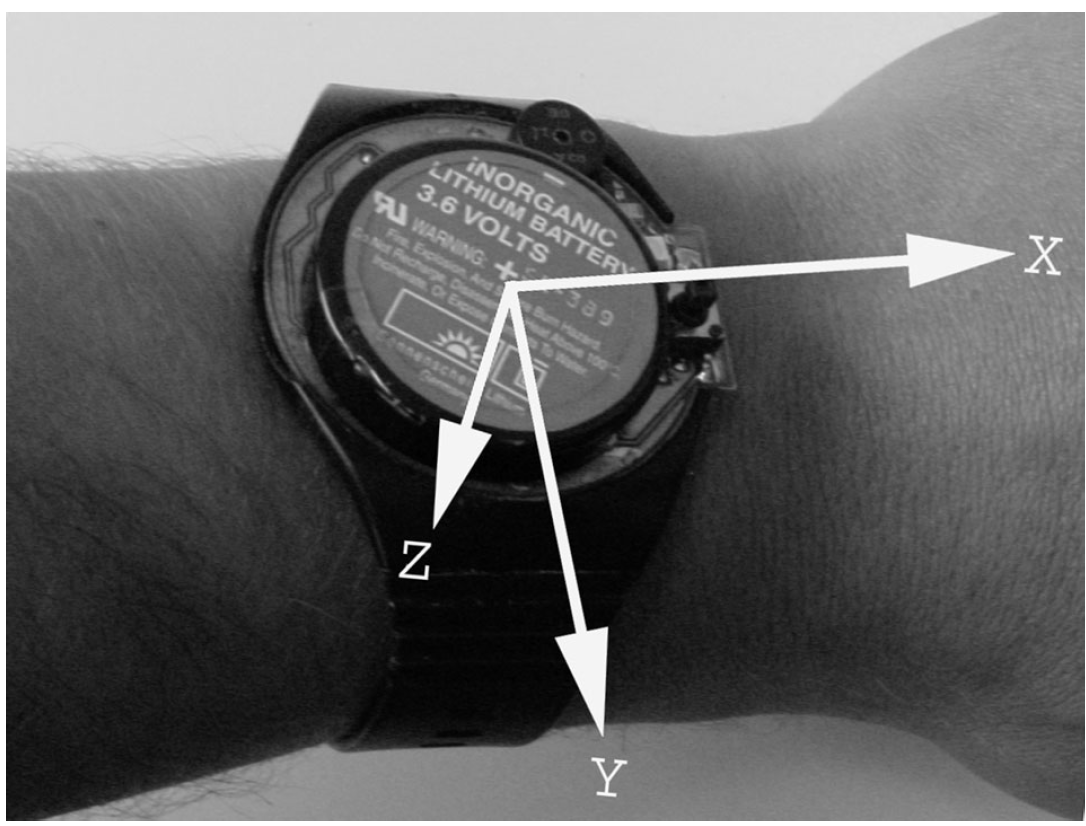
\includegraphics[scale=0.5]{imagens/speedy.png}
	\caption{ SPEEDY e seus eixos \cite{degen2003speedy}.}
	\label{fig:speedy}
\end{figure} 

O algoritmo de detecção de quedas do Speedy utiliza um algoritmo baseado em limiares com 3 valores distintos: o valor de \ac{SMV} calculado através da formula que pode ser vista em \ref{eq:SMV}, dois valores de velocidade distintos chamados de $v_1$ e $v_2$. A velocidade $v_1$ é o valor aproximado da velocidade vertical (de queda), e o valor da velocidade $v_2$ representa a velocidade do dispositivo Speedy. 

No primeiro passo do algoritmo, um alto valor de velocidade precisa ser identificado indicando uma possível queda. Depois disso, nos próximos 3 segundos um impacto precisa ser detectado, representado por alto valores de aceleração. Depois disso, o usuário é observado por mais 60 segundos, se durante este tempo, pelo menos 40 segundos forem marcados por inatividade um alerta sonoro é emitido. 

O Speedy foi avaliado através de quedas simuladas por 3 individuos diferentes em um colchão. Cada indivíduo simulou  quedas em 3 posições diferentes: Frente, lado, costas. Foram realizadas um total de 45 quedas, onde 65\% delas foram corretamente marcadas como um evento de queda. 

\subsection{F2D - Sistema de Detecção de Quedas}
\label{subsec:F2D_System}
F2D é uma applicação Android embarcado em um smartwatch \textit{AW-420.RX} da Simvalley Mobile\footnote{http://www.simvalley-mobile.de/} \citep{kostopoulos2015f2d}. O algoritmo implementado no F2D tem como entrada os dados do acelerômetro, levando em consideração os movimentos realizados depois de um evento de queda e a localização do usuário. 

Para que se possa detectar as quedas, o F2D utiliza um algoritmo baseado em limiares, onde os limiares foram definidos utilizando um banco de dados com mais de 150 eventos simulados de queda. O algoritmo de detecção de quedas presente no F2D é composto de quatro etapas\citep{kostopoulos2015f2d}:

\begin{enumerate}
	
	\item{\textbf{Padrão de Queda}: Para que um evento possa ser identificado como uma possível queda, o valor da aceleração precisa ultrapassar um limite que varia de $10 m/s^{2}$ a $18 m/s^{2}$ que representa o impacto da queda, e depois de um intervalo de tempo, precisa ultrapassar um limiar de $2 m/s^{2}$  a $7 m/s^{2}$, caracterizado como o movimento residual da queda. Tanto os valores exatos dos limiares, quanto o intervalo de tempo entre a análise dos mesmos variam de acordo com perfil do usuário.   }
	
	\item{\textbf{Módulo de Decisão}: Toda vez que ambas as condições da etapa anterior são satisfeitas é acrescido 1 em um contador. São estabelecidos dois valores $X$ e $Y$. O valor de $X$ representa o limiar do contador e $Y$ representa o seu limite. Sendo assim, o valor do contador precisa ficar entre X e Y, ou seja, $ X \leq Contador < Y $. Caso este valor seja maior que Y, outra atividade estava sendo desempenhada, como por exemplo correr, e caso este valor do contador seja menor que X, onde $X = 1$, então um movimento brusco do braço aconteceu, mas que não caracteriza uma queda.  }
	
	\item{\textbf{Ação posterior a Queda}: Logo depois que um evento é caracterizado como queda, o F2D é capaz de identificar se o usuário conseguiu se recuperar, e volto a exercer suas atividades normais, caso isto ocorra, o sistema não irá emitir um alerta para o seu cuidador, caso contrário, um alerta é emitido }
	
	\item{\textbf{Ação baseada na Localização}: O F2D também se baseia na localização do usuário. Caso este esteja na rua, e todas as etapas anteriores se concretizaram, um alarme é enviado para o cuidador. Caso o usuário esteja em casa, o sistema faz uso da tecnologia \textit{iBeacon} para categorizar certos locais como seguros ou potencialmente perigosos. O iBeacon utiliza o sistema de detecção de proximidade do \ac{BLE} para enviar um identificador único para aplicações ou sistemas operacionais compatíveis que estejam ao alcance do mesmo \citep{kostopoulos2015f2d}.  Caso o local esteja marcado como potencialmente perigoso, uma mensagem é enviada ao cuidador, caso contrário, o usuário terá a oportunidade de cancelar o envio, em um possível evento de queda.}     
	
	
\end{enumerate}


\subsection{Sistema de Detecção de Quedas de Pulso}
O sistema proposto por \cite{hsieh2014wrist} utiliza dois dispositivos vestíveis acoplados no pulso do usuário como pode ser visto na figura \ref{fig:wrist_worn}. 


\begin{figure}[ht]
	\centering
	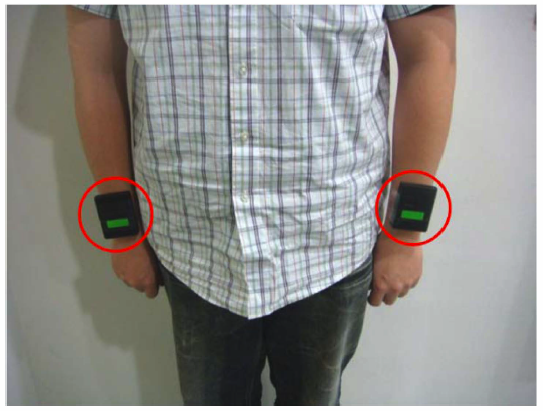
\includegraphics[scale=0.4]{imagens/wrist_worn.png}
	\caption{ Dispositivos véstiveis marcados em vermelho. \cite{hsieh2014wrist}.}
	\label{fig:wrist_worn}
\end{figure} 


Cada um dos dispositivos está equipado com um módulo Zigbee\footnote{http://www.zigbee.org/} responsável pela transmissão dos dados e  um acelerômetro e  giroscópio de 3 eixos. A frequência tanto do acelerômetro quanto do giroscópio foram configuradas para $50 Hz$, ou seja, os dados são coletados a cada \textit{20 ms}.


O algoritmo proposto utiliza ambos os dados do acelerômetro e do giroscópio para realizar a detecção de quedas. Os dados do giróscopio funcionam como um filtro inicial, desconsiderando a maioria das ativididades cotidianas, enquanto os dados do acelerômetro são responsáveis por realizar o julgamento final. O algoritmo utilizado, assim como os demais, é baseado em limiares onde os limiares foram definidos atravês de um treinamento inicial. 

O algoritmo proposto é capaz de diferenciar \ac{ADL} como bater palmas e deitar-se, de um evento de queda em 95\% dos casos. A principal desvantagem do sistema proposto é a necessidade de se utilizar 2 dispositivos, podendo torna-se desconfortável para o usuário.







